\begin{frame}
 \centerline{\Large Old Stuff}
\end{frame}



\frame{
  \frametitle{First example -- Lorenz system}
  \lstinputlisting{snippets/example1_a.cpp}

  \begin{itemize}
  \item The r.h.s. of the ODE is a simple function
  \item Observer
  \end{itemize}
}

\begin{frame}[fragile]{Lorenz system continued}
  % \lstinputlisting{snippets/example1_b.cpp}

  Different steppers:

  \begin{lstlisting}
runge_kutta4< state_type > stepper;
  \end{lstlisting}

  \pause
  
  \begin{lstlisting}
controlled_runge_kutta< runge_kutta_cash_karp54< state_type > > stepper;
  \end{lstlisting}

  \pause

  \begin{lstlisting}
dense_output_runge_kutta< controlled_runge_kutta<
    runge_kutta_dopri5< state_type > > > stepper;
  \end{lstlisting}

  \pause

  \begin{lstlisting}
runge_kutta_dopri5< state_type > stepper;
make_dense_output( 1.0e-6 , 1.0e-6 , stepper );    // incomplete
  \end{lstlisting}

  \pause

  All together:

  \begin{lstlisting}
int main( int argc , char **argv )
{
    state_type x = {{ 10.0 , 1.0 , 1.0 }};
    runge_kutta_dopri5< state_type > stepper;
    integrate_const( make_dense_output( 1.0e-6 , 1.0e-6 , stepper )
                     lorenz , x , 0.0 , 10.0 , 0.01 , write_lorenz );
    return 0;
}
  \end{lstlisting}



  
\end{frame}

\rem{
\frame{
  \frametitle{Side note: Templates}

  \begin{itemize}
  \item Programming paradigm: Generic programming
  \item Provide a mechanism that classes and functions work on arbitrary types
  \item Static (compile-time) polymorphism
  \item Good performance -- Compiler can optimize
  \item No virtual functions and runtime-polymorphy in odeint
  \item Concepts -- Description of requirements on the used types and classes
  \item Disadvantage: Long compilation time and memory consumption of the compiler
  \end{itemize}
}
}



\begin{frame}[fragile]{Second example -- Fermi-Pasta-Ulam lattice}
 
  \vspace{-4ex} 
 
  \begin{eqnarray}
   \dot{q}_k & = & p_k  \nonumber \\
   \dot{p}_k & = & - q_k^2 + \Delta q_k + \beta \big\{ ( q_{k+1} - q_k )^3 - ( q_k - q_{k-1} )^3 \big\} \nonumber
  \end{eqnarray}

  \centerline{\rem{Discrete Laplacian} $\Delta q_k = q_{k+1} -2 q_k + q_{k-1}$}

  \vspace{4ex}

  \pause

State type consists of coordinates $q$ and momentas $p$

  \vspace{1ex}

  \begin{lstlisting}
typedef std::vector<double> vector_type;
vector_type q( 256 ) , p( 256 );
// initialize q,p
std::pair< state_type , state_type > state = std::make_pair( q , p );
  \end{lstlisting}

  \pause

  \vspace{2ex}

  Hamiltonian system $\Longrightarrow{}$ Symplectic solvers needed

  \vspace{1ex}

  \begin{lstlisting}
symplectic_rkn_sb3a_mclachlan< vector_type > stepper;
  \end{lstlisting}


\end{frame}

\begin{frame}[fragile]{Fermi-Pasta-Ulam lattice continued}

  Trivial first component $\dot{q}_k = p_k$

  \begin{lstlisting}
struct fpu {
    double m_beta;
    fpu(double beta) : m_beta(beta) { }

    void operator()(const vector_type &q, vector_type &dpdt) const {
        // ...
    }
};
  \end{lstlisting}

  \pause

  \vspace{2ex}

  All together

  \begin{lstlisting}
struct statistics_observer {
    void operator()( const state_type &x , double t ) const { 
    // write the statistics
    }
};

int main(int argc, char **argv)
{
    vector_type q( 256 ) , p( 256 );
    // initialize q,p
    integrate_const( symplectic_rkn_sb3a_mclachlan< state_type >(), fpu(1.0),
        make_pair( q , p ), 0.0, 10.0, 0.01, statistics_observer() );
    return 0;
}
  \end{lstlisting}



\end{frame}



%\section{odeint details}

\frame{\tableofcontents[currentsection]}


\frame{
  \frametitle{Structure of odeint}

  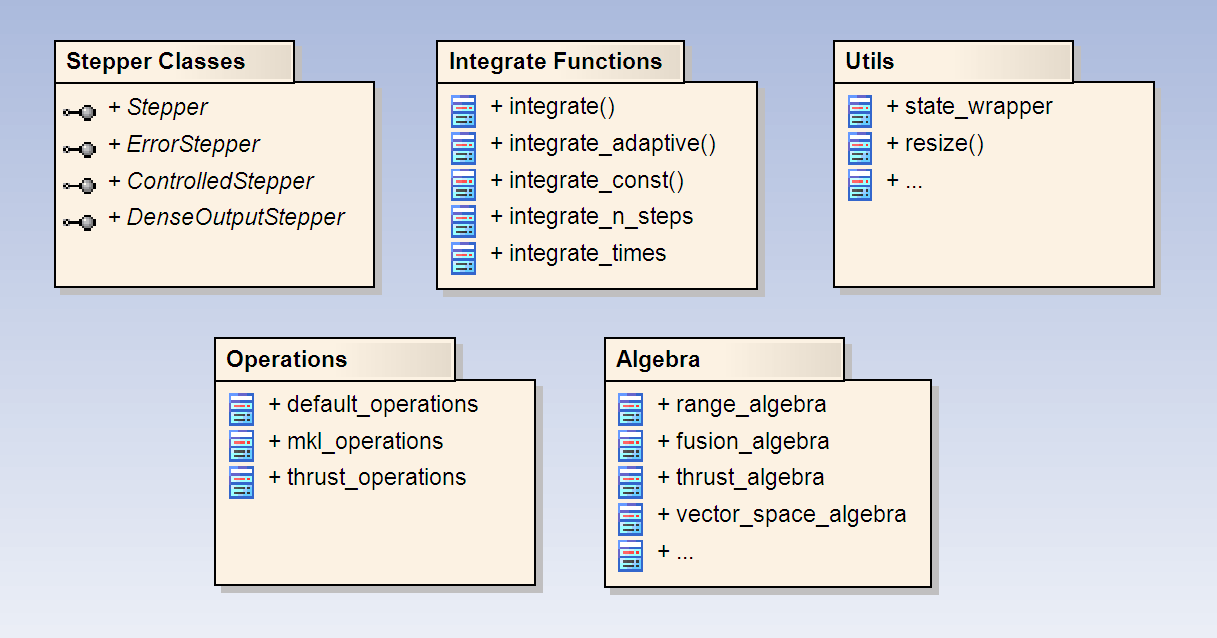
\includegraphics[draft=false,width=1.0\textwidth]{odeint_components.png}

}



\begin{frame}[fragile]
  \frametitle{Internals -- Example Euler's method}

User provides 
  \begin{displaymath}
    y_i = f_i( x(t) , t ) % \,\,\textrm{,} \quad \textrm{for all} \quad i \in (1,\dots,N)
  \end{displaymath}

odeint provides
  \begin{displaymath}
    x_i (t + \Delta t ) = x_i( t )  + \Delta t \cdot y_i
  \end{displaymath}

(In general vector operations like $\,\, z_i = a_1 x_{1,i} + a_2 x_{2,i} + \dots $)



\vspace{4ex}

Instantiation

\vspace{1ex}

\begin{lstlisting}[basicstyle=\small\ttfamily,escapechar=!]
euler<state_type, value_type, deriv_type, time_type, algebra, operations > stepper;
\end{lstlisting}

\vspace{1ex}

{\bf All elements for container independence and portability are already included in this line!}

\end{frame}

\begin{frame}[fragile]
  \frametitle{Internals -- Example Euler's method}

  \begin{displaymath}
    y_i = f_i( x(t) )
  \end{displaymath}
  \begin{displaymath}
    x_i (t + \Delta t ) = x_i( t )  + \Delta t \cdot y_i
  \end{displaymath}

\vspace{2ex}

\begin{lstlisting}[basicstyle=\small\ttfamily]
euler<state_type, value_type, deriv_type, time_type, algebra, operations > stepper;
\end{lstlisting}

\vspace{2ex}

\begin{overlayarea}{\textwidth}{10cm}
 \rem{\only<1>{General goal: Separation 
  \begin{itemize}
   \item of how an vector is iterated
   \item of how the basic computations are performed
  \end{itemize}
from the stepper
 }}
\rem{ \only<1>{Examples:

  {\tt \scriptsize euler<vector<double>, double, vector<double>, double ,
range\_algebra, default\_operations>;}

\vspace{1ex}

  {\tt \scriptsize euler<vector<complex<double> >, double, vector<complex<double> >, double ,
range\_algebra, default\_operations>;}  

  {\tt \scriptsize euler<thurst::device\_vector<double>, double, thrust::device\_vector<double>, double ,
thrust\_algebra, thrust\_algebra>;} 
}}
 \only<1>{
 Data types
 \begin{itemize}
  \item {\tt state\_type} -- the type of $x$
  \item {\tt value\_type} -- the basic numeric type, e.g. {\tt double}
  \item {\tt deriv\_type} -- the type of $y$
  \item {\tt time\_type} -- the type of $t$, $\Delta t$
 \end{itemize}}
 \only<2>{
 Algebra policies, perform the iteration

 \vspace{2ex}

 Algebra must be a class with public methods
 \begin{itemize}
 \item {\tt for\_each1(x,op)} -- Performs $op(x_i)$ for all $i$
 \item {\tt for\_each2(x1,x2,op)} -- Performs $op(x1_i,x2_i)$ for all $i$
 \item ...
 \end{itemize}}
 \only<3>{
 Operations do the basic computation

 \vspace{2ex}

 Operations must be a class with the public classes (functors)
 \begin{itemize}
 \item {\tt scale\_sum1} -- Calculates $x = a1 \cdot y1 $
 \item {\tt scale\_sum2} -- Calculates $x = a1 \cdot y1 + a2 \cdot y2$
 \item ...
 \end{itemize}}
 \only<4>{
 All together

\vspace{2ex}
   {\tt \scriptsize m\_algebra.for\_each3(xnew ,xold, y ,\\
\hspace{4ex}operations\_type::scale\_sum2<value\_type,time\_type>(1.0,dt));}
}
\end{overlayarea}


\end{frame}




\frame{
  \frametitle{Stepper concepts}

  \begin{block}{Concepts}
    ``... In generic programming, a concept is a description of supported
    operations on a type...''
  \end{block}

  \pause
  \vspace{4ex}
  odeint provides
  \begin{itemize}
   \item Stepper concept \\ \lstinline[basicstyle=\small\ttfamily]+stepper.do_step(sys,x,t,dt);+
   \item ErrorStepper concept \\ \lstinline[basicstyle=\small\ttfamily]+stepper.do_step(sys,x,t,dt,xerr);+
   \item ControlledStepper concept \\ \lstinline[basicstyle=\small\ttfamily]+stepper.try_step(sys,x,t,dt);+
   \item DenseOutputStepper concept \\ \lstinline[basicstyle=\small\ttfamily]+stepper.do_step(sys);+ \\ \lstinline[basicstyle=\small\ttfamily]+stepper.calc_state(t,x);+
  \end{itemize}

}

\rem{
\frame{
  \begin{block}{Concepts}
    ``... In generic programming, a concept is a description of supported
    operations on a type...''
  \end{block}
  \begin{columns}[t]
    \begin{column}{0.32\textwidth}
      \begin{block}{Stepper}
        {\footnotesize
          provides method:
          {do\_step(sys,x,t,dt)}

        \vspace{1ex}

        Performs one time step with constant step size

        \vspace{1ex}

        Example:

        stepper\_rk4<vector>~rk;

        ...

        rk.do\_step(lor,x,t,dt);
        }
      \end{block}
    \end{column}
    \begin{column}{0.32\textwidth}
      \begin{block}{Error stepper}
        {\footnotesize
          provides method:
          {do\_step(sys,x,t,dt,xerr)}

        \vspace{1ex}

        Performs one time step with constant step size and error estimation

        \vspace{1ex}

        Example:

        stepper\_rk5\_ck<..>~rk;

        ...

        rk.do\_step(lor,x,t,dt,xerr);}
      \end{block}
    \end{column}
    \begin{column}{0.32\textwidth}
      \begin{block}{Controlled stepper}
        {\footnotesize
          provides method:
          {try\_step(sys,x,t,dt)}

        \vspace{1ex}

        Tries to performs one time step within a given accuracy. Suggests new
        step size.

        \vspace{1ex}

        Example:

        controlled\_stepper\_bs;
        }
      \end{block}
    \end{column}
  \end{columns}

  Dense output concept
}
}

\frame{
  \frametitle{Supported methods}
    {\scriptsize
    \begin{tabular}{lll}
      {\bf Method} & {\bf Class name} & {\bf Concept} \\
      Euler & {\tt euler} & SD \\
      Runge-Kutta 4 & {\tt runge\_kutta4} & S \\
      Runge-Kutta Cash-Karp & {\tt runge\_kutta\_cash\_karp54} & SE \\
      Runge-Kutta Fehlberg & {\tt runge\_kutta\_runge\_fehlberg78} & SE \\
      Runge-Kutta Dormand-Prince & {\tt runge\_kutta\_dopri5} & SED \\
      & & \\
      Runge-Kutta controller & {\tt controlled\_runge\_kutta} & C \\
      Runge-Kutta dense output & {\tt dense\_output\_runge\_kutta} & D \\
      & & \\
      Symplectic Euler & {\tt symplectic\_euler} & S \\
      Symplectic RKN & {\tt symplectic\_rkn\_sb3a\_mclachlan} & S \\
      & & \\
      Rosenbrock 4 & {\tt rosenbrock4} & ECD \\
      Implicit Euler & {\tt implicit\_euler} & S \\
      & & \\
      Adams-Bashforth-Moulton & {\tt adams\_bashforth\_moulton} & S \\
      Bulirsch-Stoer & {\tt bulirsch\_stoer} & CD 
    \end{tabular}

    \vspace{4ex}

    S -- fulfills stepper concept

    E -- fulfills error stepper concept

    C -- fulfills controlled stepper concept

    D -- fulfills dense output stepper concept

  }
}






\frame{
  \frametitle{Integrate functions}

  \begin{itemize}
   \item {\tt integrate\_const}
   \item {\tt integrate\_adaptive}
   \item {\tt integrate\_times}
   \item {\tt integrate\_n\_steps}
  \end{itemize}

  Perform many steps, use all features of the underlying method

  \vspace{2ex}

  \pause

  An additional observer can be called

  \vspace{2ex}

  {\tt integrate\_const(stepper, sys, x, t\_start, t\_end, dt, obs);}

}





\frame{
  \frametitle{More internals}
    \begin{itemize}
      \item Header-only, no linking $\rightarrow$ powerful compiler optimization
      \item Memory allocation is managed internally
      \item No virtual inheritance, no virtual functions are called
      \item Different container types are supported, for example
        \begin{itemize}
          \item STL containers ({\tt vector}, {\tt list}, {\tt map}, {\tt tr1::array})
          \item MTL4 matrix types, blitz++ arrays, Boost.Ublas matrix types
          \item {\tt thrust::device\_vector}
          \item Fancy types, like Boost.Units
          \item ANY type you like
        \end{itemize}
      \item Explicit Runge-Kutta-steppers are implemented with a new template-metaprogramming method
      \item Different operations and algebras are supported
        \begin{itemize}
          \item MKL
          \item Thrust
          \item gsl
        \end{itemize}
    \end{itemize}
}


\frame{
  \frametitle{ODEs on GPUs}

  Graphical processing units (GPUs) are able to perform up to $10^6$ operations at once in parallel
 
  \vspace{2ex}

  Frameworks
  \begin{itemize}
   \item CUDA from NVIDIA
   \item OpenCL
   \item Thrust a STL-like library for CUDA and OpenMP
  \end{itemize}

  \vspace{2ex}

  Applications:
  \begin{itemize}
   \item Parameter studies
   \item Large systems, like ensembles or one- or two dimensional lattices
   \item Discretizations of PDEs
  \end{itemize}

  \vspace{2ex}

  {\bf odeint supports CUDA, through Thrust}
}

\frame{
  \frametitle{Example: Parameter study of the Lorenz system}

  \lstinputlisting{snippets/example3_thrust.cpp}
}




%\section{Outlook and conclusion}

\frame{
  \frametitle{Conclusion}

  \begin{itemize}
    \item odeint provides a fast, flexible and easy-to-use C++ library for
      numerical integration of ODEs.
    \item Its container independence is a large advantage over existing
      libraries.
    \item Portable
    \item Generic programming is the main programming technique.
  \end{itemize}

}



\frame{
  \frametitle{Outlook}
  \begin{itemize}
    \item Submission to the boost libraries
    \item Dynamical system classes for easy implementation of interacting dynamical systems
    \item More methods: implicit methods and multistep methods.
    \item Implementation of the Taylor series method
  \end{itemize}

  \vspace{4ex}

  \lstinputlisting{snippets/example4_lorenz_taylor.cpp}
}



\frame{
  \frametitle{Resources}

Download and documentation

{\tt odeint.com}

\vspace{2ex}

An article about the used techniques exists at

{\tt \small http://www.codeproject.com/KB/recipes/odeint-v2.aspx}

\vspace{2ex}

Development

{\tt https://github.com/headmyshoulder/odeint-v2}

\vspace{4ex}

\begin{block}{Contributions and feedback}
 are highly welcome
\end{block}





}
